\documentclass[11pt]{article}
\usepackage{graphicx}
\graphicspath{ {./pictures/} }

\usepackage[hoptionsi]{subcaption}

%%%%%%%%%%%%%%%%%%%%%%%%%%%%%%%%%%%%%%%%%
% Lachaise Assignment
% Structure Specification File
% Version 1.0 (26/6/2018)
%
% This template originates from:
% http://www.LaTeXTemplates.com
%
% Authors:
% Marion Lachaise & François Févotte
% Vel (vel@LaTeXTemplates.com)
%
% License:
% CC BY-NC-SA 3.0 (http://creativecommons.org/licenses/by-nc-sa/3.0/)
% 
%%%%%%%%%%%%%%%%%%%%%%%%%%%%%%%%%%%%%%%%%

%----------------------------------------------------------------------------------------
%	PACKAGES AND OTHER DOCUMENT CONFIGURATIONS
%----------------------------------------------------------------------------------------

\usepackage{amsmath,amsfonts,stmaryrd,amssymb} % Math packages

\usepackage{enumerate} % Custom item numbers for enumerations

\usepackage[ruled]{algorithm2e} % Algorithms

\usepackage[framemethod=tikz]{mdframed} % Allows defining custom boxed/framed environments

\usepackage{listings} % File listings, with syntax highlighting
\lstset{
	basicstyle=\ttfamily, % Typeset listings in monospace font
}

%----------------------------------------------------------------------------------------
%	DOCUMENT MARGINS
%----------------------------------------------------------------------------------------

\usepackage{geometry} % Required for adjusting page dimensions and margins

\geometry{
	paper=a4paper, % Paper size, change to letterpaper for US letter size
	top=2.5cm, % Top margin
	bottom=3cm, % Bottom margin
	left=2.5cm, % Left margin
	right=2.5cm, % Right margin
	headheight=14pt, % Header height
	footskip=1.5cm, % Space from the bottom margin to the baseline of the footer
	headsep=1.2cm, % Space from the top margin to the baseline of the header
	%showframe, % Uncomment to show how the type block is set on the page
}

%----------------------------------------------------------------------------------------
%	FONTS
%----------------------------------------------------------------------------------------

\usepackage[utf8]{inputenc} % Required for inputting international characters
\usepackage[T1]{fontenc} % Output font encoding for international characters

\usepackage{XCharter} % Use the XCharter fonts

%----------------------------------------------------------------------------------------
%	COMMAND LINE ENVIRONMENT
%----------------------------------------------------------------------------------------

% Usage:
% \begin{commandline}
%	\begin{verbatim}
%		$ ls
%		
%		Applications	Desktop	...
%	\end{verbatim}
% \end{commandline}

\mdfdefinestyle{commandline}{
	leftmargin=10pt,
	rightmargin=10pt,
	innerleftmargin=15pt,
	middlelinecolor=black!50!white,
	middlelinewidth=2pt,
	frametitlerule=false,
	backgroundcolor=black!5!white,
	frametitle={Command Line},
	frametitlefont={\normalfont\sffamily\color{white}\hspace{-1em}},
	frametitlebackgroundcolor=black!50!white,
	nobreak,
}

% Define a custom environment for command-line snapshots
\newenvironment{commandline}{
	\medskip
	\begin{mdframed}[style=commandline]
}{
	\end{mdframed}
	\medskip
}

%----------------------------------------------------------------------------------------
%	FILE CONTENTS ENVIRONMENT
%----------------------------------------------------------------------------------------

% Usage:
% \begin{file}[optional filename, defaults to "File"]
%	File contents, for example, with a listings environment
% \end{file}

\mdfdefinestyle{file}{
	innertopmargin=1.6\baselineskip,
	innerbottommargin=0.8\baselineskip,
	topline=false, bottomline=false,
	leftline=false, rightline=false,
	leftmargin=2cm,
	rightmargin=2cm,
	singleextra={%
		\draw[fill=black!10!white](P)++(0,-1.2em)rectangle(P-|O);
		\node[anchor=north west]
		at(P-|O){\ttfamily\mdfilename};
		%
		\def\l{3em}
		\draw(O-|P)++(-\l,0)--++(\l,\l)--(P)--(P-|O)--(O)--cycle;
		\draw(O-|P)++(-\l,0)--++(0,\l)--++(\l,0);
	},
	nobreak,
}

% Define a custom environment for file contents
\newenvironment{file}[1][File]{ % Set the default filename to "File"
	\medskip
	\newcommand{\mdfilename}{#1}
	\begin{mdframed}[style=file]
}{
	\end{mdframed}
	\medskip
}

%----------------------------------------------------------------------------------------
%	NUMBERED QUESTIONS ENVIRONMENT
%----------------------------------------------------------------------------------------

% Usage:
% \begin{question}[optional title]
%	Question contents
% \end{question}

\mdfdefinestyle{question}{
	innertopmargin=1.2\baselineskip,
	innerbottommargin=0.8\baselineskip,
	roundcorner=5pt,
	nobreak,
	singleextra={%
		\draw(P-|O)node[xshift=1em,anchor=west,fill=white,draw,rounded corners=5pt]{%
		Question \theQuestion\questionTitle};
	},
}

\newcounter{Question} % Stores the current question number that gets iterated with each new question

% Define a custom environment for numbered questions
\newenvironment{question}[1][\unskip]{
	\bigskip
	\stepcounter{Question}
	\newcommand{\questionTitle}{~#1}
	\begin{mdframed}[style=question]
}{
	\end{mdframed}
	\medskip
}

%----------------------------------------------------------------------------------------
%	WARNING TEXT ENVIRONMENT
%----------------------------------------------------------------------------------------

% Usage:
% \begin{warn}[optional title, defaults to "Warning:"]
%	Contents
% \end{warn}

\mdfdefinestyle{warning}{
	topline=false, bottomline=false,
	leftline=false, rightline=false,
	nobreak,
	singleextra={%
		\draw(P-|O)++(-0.5em,0)node(tmp1){};
		\draw(P-|O)++(0.5em,0)node(tmp2){};
		\fill[black,rotate around={45:(P-|O)}](tmp1)rectangle(tmp2);
		\node at(P-|O){\color{white}\scriptsize\bf !};
		\draw[very thick](P-|O)++(0,-1em)--(O);%--(O-|P);
	}
}

% Define a custom environment for warning text
\newenvironment{warn}[1][Warning:]{ % Set the default warning to "Warning:"
	\medskip
	\begin{mdframed}[style=warning]
		\noindent{\textbf{#1}}
}{
	\end{mdframed}
}

%----------------------------------------------------------------------------------------
%	INFORMATION ENVIRONMENT
%----------------------------------------------------------------------------------------

% Usage:
% \begin{info}[optional title, defaults to "Info:"]
% 	contents
% 	\end{info}

\mdfdefinestyle{info}{%
	topline=false, bottomline=false,
	leftline=false, rightline=false,
	nobreak,
	singleextra={%
		\fill[black](P-|O)circle[radius=0.4em];
		\node at(P-|O){\color{white}\scriptsize\bf i};
		\draw[very thick](P-|O)++(0,-0.8em)--(O);%--(O-|P);
	}
}

% Define a custom environment for information
\newenvironment{info}[1][Info:]{ % Set the default title to "Info:"
	\medskip
	\begin{mdframed}[style=info]
		\noindent{\textbf{#1}}
}{
	\end{mdframed}
}
 % Include the file specifying the document structure and custom commands

%----------------------------------------------------------------------------------------
%	ASSIGNMENT INFORMATION
%----------------------------------------------------------------------------------------

\title{Dynamic Distributed Decision Making \\Project 1 \\MIE567} % Title of the assignment

\author{\texttt{Hao Tan 999735728}\\ \texttt{Xiali Wu 999011322} \\ \texttt{David Molina}} % Author name and email address

\date{University of Toronto --- \today} % University, school and/or department name(s) and a date

%----------------------------------------------------------------------------------------

\begin{document}

\maketitle

\section{Modelling}
\textbf{First, you are tasked with modelling the Gridworld domain
above as a Markov decision process. Then, you are asked to provide a complete
programming description of the problem that will be used to solve it
computationally.}
\\

% 1---------------------------------------------------------------
\noindent
\textbf{1}
\noindent
\textbf{Explain how you would model this navigation problem as a Markov
decision process. In particular:}
\\

% 1A---------------------------------------------------------------
\noindent
\textbf{a)}
\noindent
\textbf{Why is this problem an MDP? }
\\

\noindent
This problem can be modeled as an MDP because it has a discrete state space
(cells) and a set of actions (north, east, west, south)/(up, right, down, left),
where the transition from one state to another is based on a given action.
\\

\noindent
We can model this problem in terms of components such as a reward
function,actions, transition probability, states, time steps, discount factor.
All these components describe a MDP type of question. This problem is infinite
horizon MDP since we can take unlimited amounts of steps between cells, and
possibly revisit the same cell. Unlimited amount steps are definitely not
optimal , but can potentially happen to max reward. Therefore, for infinite
horizon MDP, a discount factor accounts for future reward.
\\

\noindent
Based on the definition of Markovian property, a stochastic process has the
Markov property if the conditional probability distribution of future states of
the process (conditional on both past and present states) depends only upon the
present state, not on the sequence of events that preceded it (ie. P[St+1 | St]
= P[St+1 | S1, S2 ... St]). In the given problem description, since the agent
can only move one cell for one action, the next cell is only dependent on the
current cell; the next cell is not depending on all previous cell before the
current cell.
\\

% 1B---------------------------------------------------------------
\noindent
\textbf{b)}
\noindent
\textbf{What are suitable state and action spaces for this problem? Are
these the only possible choices? Why or why not?}
\\

\noindent
The States can be represented as the coordinates of the grid (i,j), where i=
0,..,4, and j=0,...,4. Then, the set of states is State = {[ (0,0), (0,1),
(0,2), (0,3), (0,4), (1,0), (1,1), (1,2), (1,3), (1,4), (2,0), (2,1), (2,2),
(2,3), (2,4), (3,0), (3,1), (3,2), (3,3), (3,4), (4,0), (4,1), (4,2), (4,3),
(4,4)]}.
\\

\begin{figure}[h]
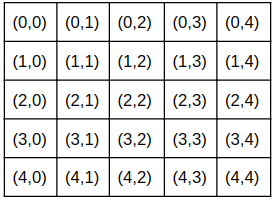
\includegraphics[scale=0.5]{states}
\centering
\caption{States represented in coordinate format}
\end{figure}

\noindent
The available set of actions are north, east, west, south, that can be
represented as adding or subtracting to the respective coordinate, i.e Action =
{[0, 1], [0, -1], [1, 0], [-1, 0]}. [0,-1] means going west; [-1,0] means going
north; [0,1] means going east; [1,0] means going south.
\\

\noindent
There are other alternatives for the representation of this problem, for
example, each cells can be represented with a number from 1 to 25 and actions
can be represented as letters A = {N, E, W, S} or {up, right, down, left}. This
type of action representation is difficult to implement in mathematical
calculations and representation. We can’t identify the situation of off-the-grid
when moving one action.
\\

\noindent
We decided to represent it as a coordinate to facilitate coding, mathematical
calculations and visual representation of the outputs for this project. 
\\

\noindent
Diagonal action ={ [1, 1], [-1, -1], [1,-1], [-1,1]} Diagonal action requires
both coordinates to move. Therefore with the constraint of moving one cell in
one direction at a time, diagonal actions require moving two directions in order
to complete one action at a time, given only compass direction of north, east,
west, and south. This conflicts with the problem description, and therefore not
used in the model.
\\


% 1C---------------------------------------------------------------
\noindent
\textbf{c)}
\noindent
\textbf{What is the transition probability matrix P? (You may describe just
the non-zero entries.)}
\\

\noindent
Assuming a policy where each four actions has the same probability to be chosen,
then the transition probability matrix is 0.25 for all four cells surrounding
the current cell. For example, the current cell is (0,0); there is 50 \% chances
that it will go off the grid; there is 25 \% chances of moving to cell(0,1);
25\% chances of moving to cell (1,0). 
\\

\begin{figure}[h]
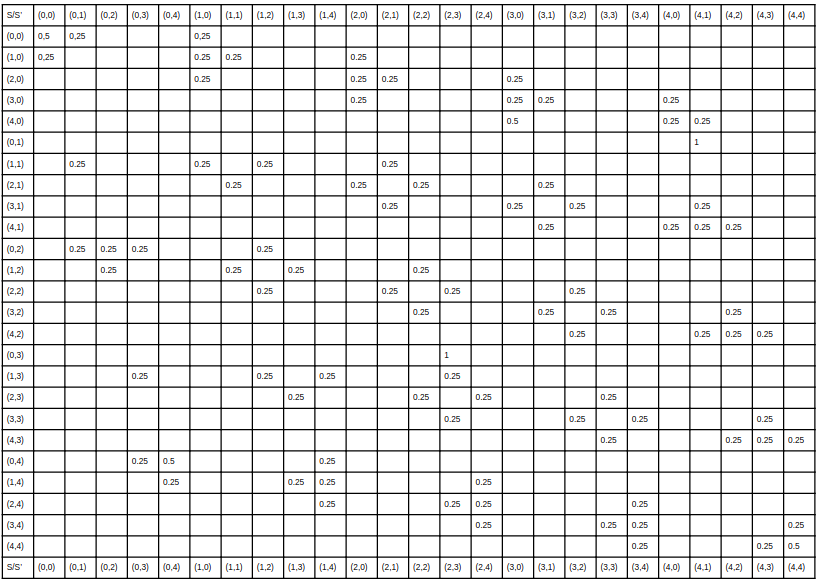
\includegraphics[scale=0.5]{transition_matrix}
\centering
\caption{Transition Matrix}
\end{figure}


% 1D---------------------------------------------------------------
\noindent
\textbf{d)}
\noindent
\textbf{Is the reward function provided the only possible one? If so, explain
why. If not, provide an example of a different reward function that would lead
to the same optimal behaviour}
\\

\noindent
The reward function = {0,-1,+5,+10} is the only possible one given the problem
description. This is the only reward function that leads to the optimal
behaviour solved below. To satisfy this reward forward, we are assuming that
when the current state is at the edge, taking East or West direction meaning the
next state is off the grid. For example, the current state is (0,4), taking East
direction leads to off-the-grid. However, without the state assumption, taking
East or West direction can mean that the next state is the last cell in the
above row, or the first cell in the next row. Take the same current state (0,4)
as an example, then taking East direction leads to (1,0). 
\\

% 1E---------------------------------------------------------------
\noindent
\textbf{e)}
\noindent
\textbf{Derive the discounted Bellman equation for the problem, and simplify
as much as you can. (Hint: to avoid deriving a separate value for each state,
try to find groups of states such that you can write a single expression for V for
them) What do you think is/are the optimal policy/policies for this problem,
and why (you do NOT need to solve the Bellman equations)?}
\\

\noindent
Since the goal is maximizing reward, optimal policy always looks for A or B to
get +10 or +5 reward. If the initial state is away from row 0 where A and B are
located, such as row 4, the optimal policy requires more actions to get to the
vicinity of A or B. If the initial state is in the vicinity of A and B, there is
a tradeoff between more actions towards A and earning discounted +5 more reward
from A->A’ compared to B->B’.
\\

% \begin{figure}[h]
% 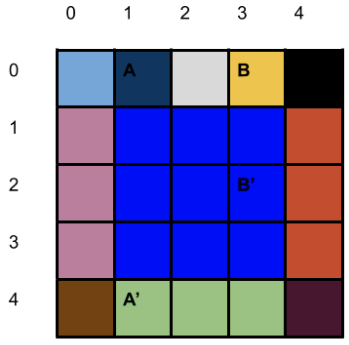
\includegraphics[scale=0.5]{bellman_groups}
% \centering
% \caption{Groups of Bellman Equations}
% \end{figure}

\begin{equation}
v_{\pi}(s)=\sum_{a} \pi(a | s) \sum_{s^{\prime}, r} p\left(s^{\prime}, r | s, a\right)\left[r+\gamma v_{\pi}\left(s^{\prime}\right)\right]
\end{equation}


% 1E BELLMAN EQUATIONS -----------------------------------------------------

\begin{equation}
\begin{array}{c}
{P([0,-1] |(i, j))(-1+\gamma v(i, j))+P[-1,0] |(i, j)(-1+\gamma v(i, j))} \\
{+P([0,+1](i, j))(0+\gamma v(i, j+1))+P([+1, 0] |(i, j))(0+\gamma v(i+1, j))} \\
{\quad \text { for } i \in\{0\}, j \in\{0\}}
\end{array}
\end{equation}

\begin{equation}
\begin{array}{c}
{P([0,-1] |(i, j))(10+\gamma v(i+4, j))+P([-1,0]|(i,j))(10+\gamma v(i+4, j))} \\
{+P([0,+1] |(i, j))(10+\gamma v(i+4, j))+P([+1,0]|(i,j))(10+\gamma v(i+4, j))} \\
{\quad \text { for } i \in\{0\}, j \in\{1\}}
\end{array}
\end{equation}

\begin{equation}
\begin{array}{c}
{P([0,-1](i, j))(0+\gamma v(i, j-1))+P([-1,0] |(i, j))(-1+\gamma v(i, j))} \\
{+P([0,+1] |(i, j))(0+\gamma v(i, j+1))+P(\tau+1,0] |(i, j))(0+\gamma v((i+1), j))} \\
{\quad \text { for } i \in\{0\}, j \in\{2\}}
\end{array}
\end{equation}

\begin{equation}
\begin{array}{c}
{P([0,-1] |(i, j))(5+\gamma v(i+2, j))+P([-1,0] |(i, j))(5+\gamma v(i+2, j))} \\
{+P([0,+1](i, j))(5+\gamma v(i+2, j))+P([+1,0] |(i, j))(5+\gamma v(i+2, j))} \\
{\quad \text { for } i \in\{0\}, j \in\{3\}}
\end{array}
\end{equation}

\begin{equation}
\begin{array}{c}
{P([0,-1] |(i, j))(-1+\gamma v(i, j))+P([-1,0] |(i, j))(0+\gamma v(i-1, j))} \\
{+P([0,+1] |(i, j))(0+\gamma v(i, j+1))+P([+1,0] |(i, j))(0+\gamma v(i+1, j))} \\
{\quad \text { for } i \in\{1,2,3\}, j \in\{0\}}
\end{array}
\end{equation}

\begin{equation}
\begin{array}{c}
{P([0,-1]|(i, j))(-1+\gamma v(i, j))+P([-1,0] /(i, j))(0+\gamma v(i-1, j))}\\
{\left.\left.+P(\left[0,+1\right] |(i, j)\right)(0+\gamma(i, j+1))+P([+1,0] |(i, j)\right)(0+\gamma v(i+1, j))}\\
{\text { for } i \in\{1,2,3\}, j \in\{0\}}
\end{array}
\end{equation}

\begin{equation}
\begin{array}{c}
{P([0,-1] |(i,j))(0+\gamma v(i, j-1))+P([-1,0] |(i, j))(0+\gamma v(i-1, j))} \\
{+P([0,+1]|(i, j)| 0+\gamma v(i, j+1))+P([+1,0] |(i, j))(0+\gamma v(i+1, j))} \\
{\quad \text { for } i \in\{1,2,3\}, j \in\{1,2,3\}}
\end{array}
\end{equation}

\begin{equation}
\begin{array}{c}
{P([0,-1]|(i, j))(0+\gamma v(i, j-1))+P([-1,0] |(i, j))(0+\gamma v(i-1, j))} \\
{+P([0,+1]|(i, j)|-1+\gamma v(i, j))+P([+1,0] |(i, j))(0+\gamma v(i+1, j))} \\
{\quad \text { for } i \in\{1,2,3\}, j \in\{4\}}
\end{array}
\end{equation}

\begin{equation}
\begin{array}{c}
{\left.P(\left[0,-1\right]|(i, j)(-1+\gamma v(i, j))+P([-1,0]|(i, j)\right)\left(0+\gamma v \left(i-1, j\right)\right)} \\
{\left.+P\left([0,+1]\right|(i, j))(0+\gamma v(i, j+1))+P([+1,0]|(i, j)|-1+\gamma v(i, j)\right)} \\
{\text{for } i \in\{4\}, j \in\{0\}}
\end{array}
\end{equation}

\begin{equation}
\begin{array}{c}
{{P\left([0,-1] |(i,j)\right](0+\gamma v(i, j-1))+P([-1,0] |(i, j))\left(0+\gamma v(i-1, j)\right)}} \\
{{\left.+P([0,+1] |(i, j)\right)(0+\gamma v(i, j+1))+P([+1,0] |(i, j))(-1+\gamma v(i, j))}}\\
{\text { for } i \in\{4\}, j \in\{1,2,3\}}
\end{array}\\
\end{equation}


\begin{equation}
\begin{array}{c}
{\left.\left.P\left([0,-1\right] |(i, j)\right)(0+\gamma v(i, j-1))+P([-1,0]|(i, j)\right)(0+\gamma v(i-1, j))} \\
{+P([0,+1]|(i, j))(1+\gamma v(i, j))+P([+1,0]|(i,j))(-1+\gamma v(i, j))} \\
{\quad \text { for } i \in\{4\}, j \in\{4\}}
\end{array}
\end{equation}


% 2---------------------------------------------------------------
\newpage
\noindent
\textbf{2}
\noindent
\textbf{Now, in a Python file called Gridworld.py, create a class that replicates
the behaviour of the MDP you formulated in the previous question. Your class
should contain four functions: one to return the initial state of the MDP, one to
return a view of all possible states, and two to return, respectively, the reward and
probability of a transition (s; a; s') from state s to state s' when taking action a.}
\\

\lstset{language=Python}
\lstset{frame=lines}
\lstset{caption={Function 1: }}
\lstset{label={lst:code_direct}}
\lstset{basicstyle=\footnotesize}
\begin{lstlisting}
    def initial_state(self):
        # randomly generate an initial state
        i = random.randint(0, len(self.states)-1)
        rand_state = self.states[i]
        return rand_state
\end{lstlisting}

\lstset{caption={Function 2: }}
\lstset{label={lst:code_direct}}
\lstset{basicstyle=\footnotesize}
\begin{lstlisting}
    def possible_states(self):
        # return the possible states
        return self.states
\end{lstlisting}

\lstset{caption={Function 3: }}
\lstset{label={lst:code_direct}}
\lstset{basicstyle=\footnotesize}
\begin{lstlisting}
    def reward(self, current_pos, action):
        # take action in current pos
        self.new_pos = np.array(current_pos) + np.array(action)
        # normally, reward = 0
        reward = 0
        # if new pos results in off the grid, return reward -1
        if -1 in self.new_pos or self.size in self.new_pos:
            reward = -1
        # if in state A, transition to state A'
        if current_pos == [0, 1]:
            reward = 10
        # if in state B, transition to state B'
        if current_pos == [0, 3]:
            reward = 5
        return reward
\end{lstlisting}


% POLICY EVALUATION---------------------------------------------------------------
\section{Policy Evaluation}
\textbf{Now, suppose the agent selects all four actions with equal probability. Use your
answers to questions 1 and 2 to write a python function, in a new file policy
evaluation.py to find the value function for this policy. You may use either an
iterative method or solve the system of equations. Show the value function you
obtained to at least four decimals.}
\\

\noindent
Following value function is generated based on equal action probability, and  =
0.99. The value function found using an iterative method is as follow:
\\

\begin{figure}[h]
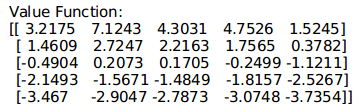
\includegraphics[scale=0.6]{v_evaluation}
\centering
\caption{Value Function using Policy Evaluation}
\end{figure}

% \begin{figure}[h]
% 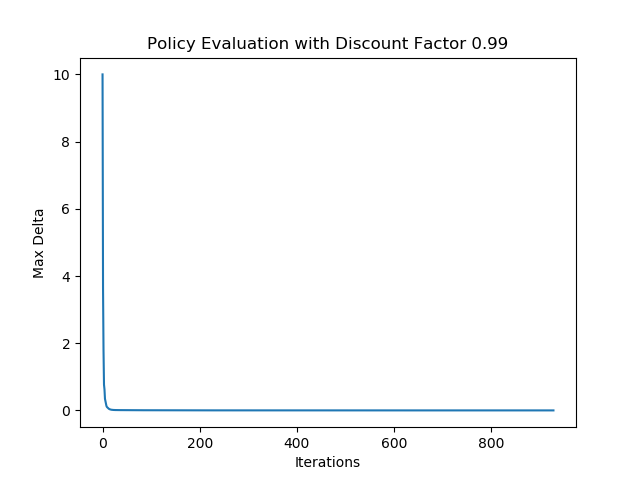
\includegraphics[scale=0.7]{policy_eval}
% \centering
% \caption{Convergence of Policy Evaluation}
% \end{figure}


% VALUE ITERATION---------------------------------------------------------------
\newpage
\section{Value Iteration}
\textbf{The goal now is to solve the MDP above using dynamic programming. In a separate
file called value iteration.py, provide a complete implementation of the value
iteration algorithm you learned in class for solving the Bellman equations you
derived earlier.}
\\

\noindent
\textbf{-}
\noindent
\textbf{Did your algorithm converge at all?}
\\

\noindent
\textbf{-}
\noindent
\textbf{How many iterations did this take for each value of $\gamma$ ?}
\\

% \begin{figure}[h]
% 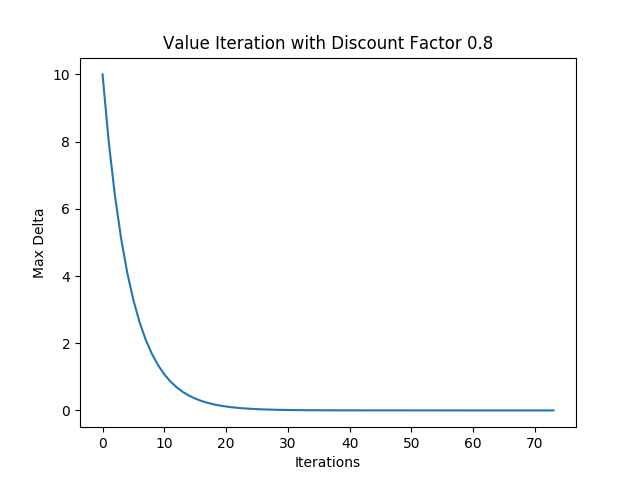
\includegraphics[scale=0.5]{Value_8}
% \centering
% \caption{Convergence of Policy Evaluation}
% \end{figure}

% \begin{figure}[h]
% 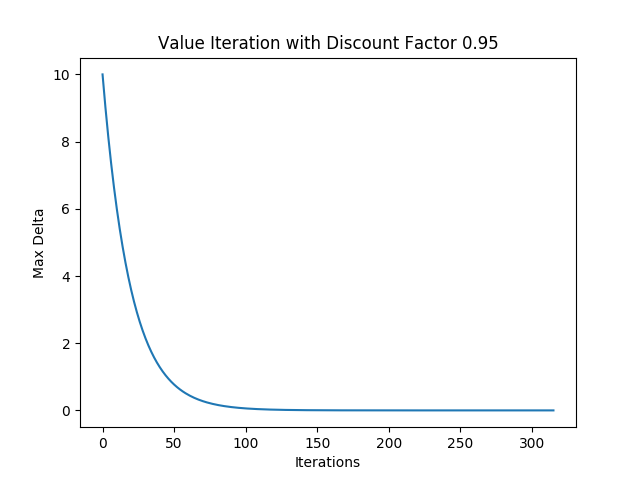
\includegraphics[scale=0.5]{Value_95}
% \centering
% \caption{Convergence of Policy Evaluation}
% \end{figure}

% \begin{figure}[h]
% 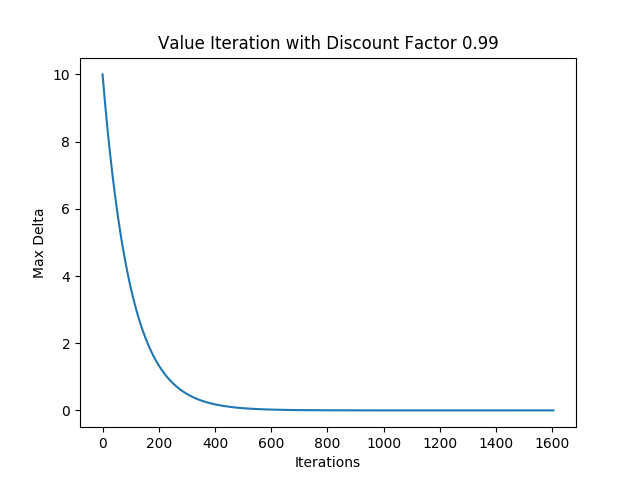
\includegraphics[scale=0.5]{Value_99}
% \centering
% \caption{Convergence of Policy Evaluation}
% \end{figure}

\noindent
\textbf{-}
\noindent
\textbf{What is the best value of $\gamma$? Also, What was the final policy you
obtained for each value of $\gamma$?}
\\

\noindent
\textbf{-}
\noindent
\textbf{Does the optimal policy you obtained correspond to the policy you
conjectured earlier?}
\\


% POLICY ITERATION---------------------------------------------------------------
\newpage
\section{Policy Iteration}
\textbf{Repeat the previous part of the assignment, but now implement the policy
iteration algorithm from class in a file called policy iteration.py. Report your
results and answer all questions as in the previous part.}
\\

\noindent
\textbf{-}
\noindent
\textbf{Did your algorithm converge at all?}
\\

\noindent
\textbf{-}
\noindent
\textbf{How many iterations did this take for each value of $\gamma$ ?}
\\

\noindent
\textbf{-}
\noindent
\textbf{What is the best value of $\gamma$? Also, What was the final policy you
obtained for each value of $\gamma$?}
\\

\noindent
\textbf{-}
\noindent
\textbf{Does the optimal policy you obtained correspond to the policy you
conjectured earlier?}
\\

% ALGORITHM COMPARISON---------------------------------------------------------------
\section{Comparison of Algorithms}
\textbf{In the final section of your report, you must compare the two algorithms you
implemented and their performance on the Gridworld domain, and comment on any
differences you observed. In particular, please answer at least the following
questions in your report:}
\\

\noindent
\textbf{-}
\noindent
\textbf{Compare the performance (e.g. values) of the optimal policies obtained
using value and policy iteration to the performance of the policy that chooses
an action at random (as you analyzed earlier), and comment on the difference.}
\\

\noindent
\textbf{-}
\noindent
\textbf{Were the value functions and policies you obtained, and the number of
iterations required to obtain these policies, similar between algorithms? How do
your results differ for different values of the parameter(s) (e.g. $\gamma$)?}
\\

\noindent
\textbf{-}
\noindent
\textbf{Which algorithm was more difficult to implement and why? Which algorithm
do you think would work better if the problem was scaled up?}
\\

\noindent
\textbf{-}
\noindent
\textbf{Include any additional insights, challenges, 
or important observations that you discovered while building or
 running your experiments.}
\\

\end{document}
